

\subsection{Sensor Calibration}

A checkerboard pattern was used to calibrate all three cameras to obtain both intrinsic and extrinsic parameters.  While the checkerboard pattern is not visible as variations in depth, it is nevertheless observed as variations in the reflected IR image whose pixels correspond to the depth pixels.  This enables the use of Zhang's method~\cite{Zhang2000} to calculate the intrinsic parameters including a $2$-parameter radial distortion of each camera, as well as a calculation of their relative poses.  The optical center of the color camera is used to define the world coordinates of our data.  The depth values of the depth camera are projected along their pixel rays and then rotated and translated by the pose of the depth camera, and thus recorded as $3$D points in the world coordinate system.
Therefore it is straight forward to project these points onto any of the three camera images.



\subsubsection{Depth Bias and Noise Characterization}
\label{sec:bias}

We characterized both the bias and the variance of the depth cameras as follows.
A flat printed checkerboard with a surrounding white board was positioned at a large number of poses in front of the sensor.
The pose of the checkerboard is calculated in each case using the color and IR reflectance images.
This defines a plane relative to the depth camera, which we use to calculate the ground truth depths for each pixel in the depth camera.
At each pose, we collect multiple depth images; this provides both a bias and variance measurement for each pixel at multiple depths.

Next we sought to model the depth bias as a linear function of depth.
Two parameters were fit for each pixel (a linear coefficient and an offset).
We found that the bias was close to a constant as a function of depth, although it varied across the depth image as shown in Figure~\ref{fig:Bias}.
The standard deviation of the pixel depth varied as a function of depth and roughly with the distance of the pixel from the optical center.
Estimates of the noise are shown in Figure~\ref{fig:Bias}.


In the recorded $3$D data we subtracted our estimated bias, and averaged five depth images for each record.  Hence the actual depth standard deviations for our data are $1/\sqrt{5}$ of the standard deviations shown in Figure~\ref{fig:Bias} (b) and the bias is zero.

Now we noticed that the chamber light shades blocked some of the depth camera field of view, and in doing so reflected some of the IR illumination.  This resulted in an additional bias shift which we measured and removed from the depth data. % FIXME

%\begin{figure}
%\begin{centering}
%\begin{tabular}{c }
%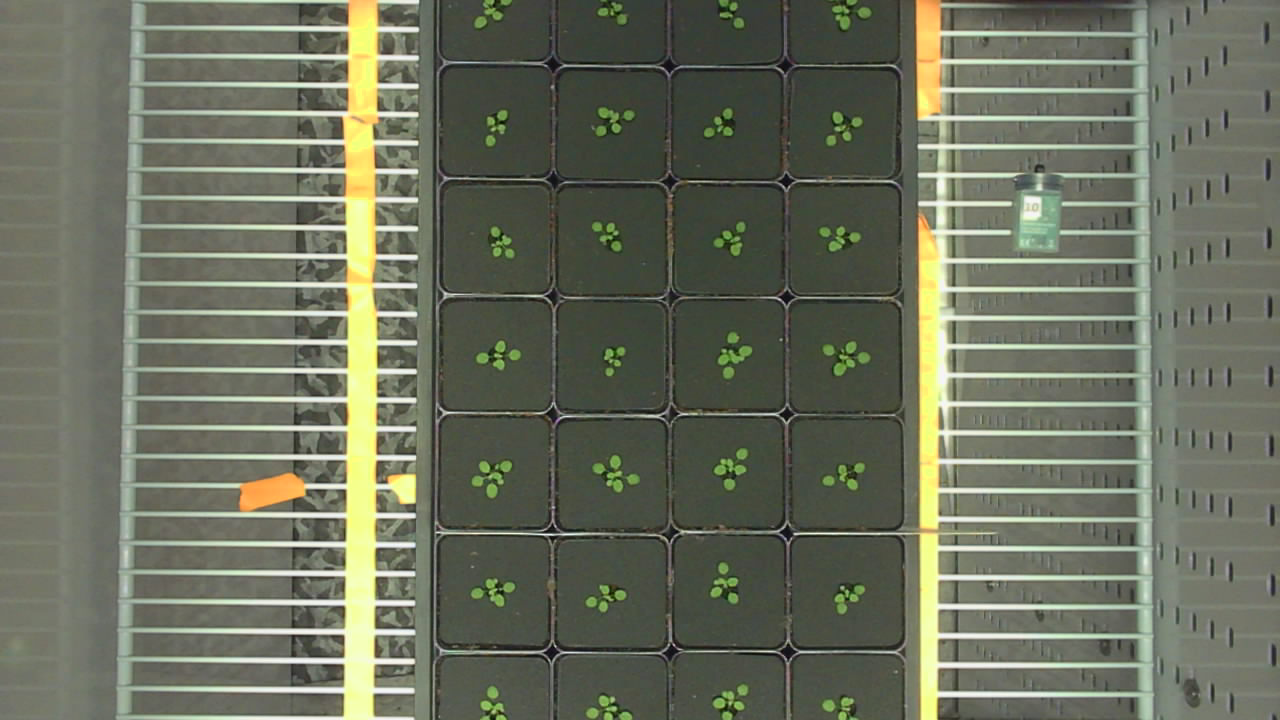
\includegraphics[width=.47\textwidth]{Figures/rawImages/a.png}\\
%Arabidopsis \\
%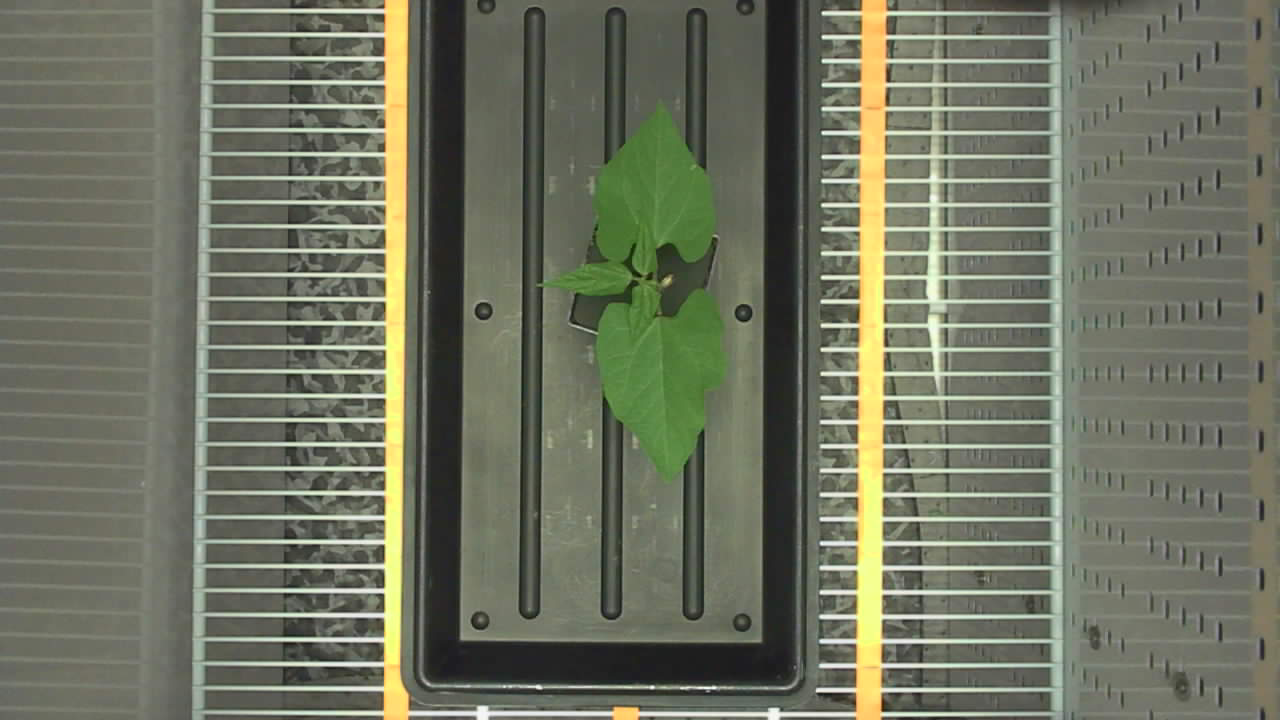
\includegraphics[width=.47\textwidth]{Figures/rawImages/b.png}\\
%   Bean \\
%\end{tabular}
%\caption{RGB color images of Arabidopsis and bean plants. }
%\label{fig:rawIm}
%\end{centering}
%\end{figure}


\begin{table*}[t!]
\begin{center}
\caption{Summary of Arabidopsis and Bean databases.}
\label{tab:stat}
\begin{tabular}{c|c|c|c|c|c}
      \hline
      % after \\: \hline or \cline{col1-col2} \cline{col3-col4} ...
      Plants     & Subjects & Days & Images/Day & Total Images & Annotated Images \\
      \hline
      Arabidopsis &  $16$      &  $9$   &     $16$     &     $2304\times 4$     &       $576\times 4$     \\
      \hline
      Bean        &   $5$      &  $5$   &     $14$     &     $350\times 4$       &       $175\times 4$  \\
      \hline
\end{tabular}
\end{center}
\end{table*}



\begin{table*}
\begin{center}
\caption{Plant image resolution of Arabidopsis and Bean databases.}
\label{tab:resolution}
\begin{tabular}{c|c|c|c|c}
      \hline
      % after \\: \hline or \cline{col1-col2} \cline{col3-col4} ...
      Plants     & Fluorescence       & IR        & RGB      & Depth     \\
      \hline
      Arabidopsis &  $\sim$$240\times240$ &  $\sim$$240\times240$  & $\sim$$120\times120$  & NA  \\
      %\hline
      Bean        & $1000\times640$ & $1000\times640$ & $380\times720$ & $90\times190$    \\
      \hline
\end{tabular}
\end{center}
\end{table*}
